\documentclass[11pt]{article}

\usepackage[a4paper,margin=1in]{geometry}
\usepackage{graphicx}
\usepackage{subcaption}
\usepackage{booktabs}
\usepackage{float}
\usepackage{amsmath}
\usepackage{hyperref}

\title{Image Denoising via Dictionary Learning}
\author{Your Name}
\date{\today}

\begin{document}

\maketitle

\section{Introduction}
Sparse dictionary learning represents image patches as sparse linear combinations of atoms from an overcomplete dictionary. In this project, the goal is to denoise grayscale natural images corrupted by zero-mean additive white Gaussian noise. Each image is divided into overlapping $8 \times 8$ patches, and each patch $y_k$ is modeled as
\[
y_k = A x_k + n_k,
\]
where $A$ is the dictionary, $x_k$ is a sparse coefficient vector, and $n_k$ is Gaussian noise. The denoised patch is reconstructed as $A x_k$, and the final denoised image is formed by averaging overlapping reconstructed patches.

\section{Brief Literature Survey}
Sparse coding is based on the idea that natural image patches admit compact representations in an overcomplete dictionary. Because structured image content is often compressible while additive Gaussian noise is not, sparse models are well suited for denoising. A key reference for this problem is the K-SVD algorithm of Aharon, Elad, and Bruckstein, which alternates between sparse coding and dictionary update steps to learn an adaptive overcomplete basis from data.

Compared with fixed transforms such as the discrete cosine transform (DCT), learned dictionaries can better match the local structures that appear in natural images, including edges, corners, and textures. This motivates the comparison between a fixed DCT+OMP baseline and a learned K-SVD+OMP model in this report. More advanced Bayesian dictionary learning approaches have also been proposed in the literature, including the multimodal sparse Bayesian formulation of Fedorov and Rao and the convergence analysis of Bayesian joint dictionary learning and sparse recovery by Joseph and Murthy. These methods are powerful, but K-SVD remains a strong and interpretable classical method for a compact course project.

\section{Dataset and Experimental Setup}
The Berkeley Segmentation Dataset (BSDS300) was used. Three grayscale images were selected uniformly at random:
\begin{itemize}
\item Image 1: \texttt{118020.jpg}
\item Image 2: \texttt{292066.jpg}
\item Image 3: \texttt{368078.jpg}
\end{itemize}

The default assignment configuration was used:
\begin{itemize}
\item patch size: $8 \times 8$
\item number of training patches: $6000$
\item number of dictionary atoms: $256$
\item sparsity level: $6$
\item K-SVD iterations: $10$
\item noise standard deviations: $\sigma \in \{5, 10, 15, 25\}$
\end{itemize}

Three methods were compared:
\begin{itemize}
\item Gaussian filtering baseline
\item fixed DCT dictionary with OMP
\item learned dictionary using K-SVD with OMP
\end{itemize}

This design gives a progression from a simple smoothing baseline to a fixed sparse representation baseline and finally to an adaptive learned sparse model. This makes it possible to test whether dictionary learning itself provides a measurable advantage over both direct filtering and a handcrafted transform dictionary.

\section{Method}
The denoising pipeline is:
\begin{enumerate}
\item Convert each image to grayscale and normalize it to a fixed working size.
\item Add Gaussian noise with a chosen standard deviation.
\item Extract overlapping $8 \times 8$ patches from the noisy image.
\item Sample $6000$ noisy patches to train a dictionary.
\item Use Orthogonal Matching Pursuit (OMP) for sparse coding.
\item Learn the dictionary using K-SVD.
\item Reconstruct the denoised image by averaging overlapping reconstructed patches.
\end{enumerate}

The final model choice was motivated by three considerations. First, the assignment is centered on dictionary learning, so a learned sparse representation model should be the main method under study. Second, OMP is a standard sparse recovery algorithm for K-SVD and is easy to interpret. Third, patch-wise averaging reduces block artifacts and gives a stable full-image reconstruction. The Gaussian and DCT baselines were retained to provide meaningful points of comparison for both classical filtering and fixed sparse coding.

\section{Assessment and Validation Procedure}
The assessment combines quantitative and qualitative evaluation. Quantitatively, the report uses mean squared error (MSE) and peak signal-to-noise ratio (PSNR). MSE directly measures the reconstruction error with respect to the clean image, while PSNR is a standard image restoration metric that is easy to compare across methods and noise levels.

The validation procedure is controlled as follows:
\begin{itemize}
\item the same three randomly selected images are used for all methods
\item the same four noise levels are used for all methods
\item the same patch size and image preprocessing are used across experiments
\item the same metrics are reported for all methods
\end{itemize}

This makes the comparison fair and isolates the effect of the denoising method itself. In addition, the assignment asks for the error as a function of noise variance, so the report summarizes the average MSE and PSNR for $\sigma^2 \in \{25, 100, 225, 625\}$.

\section{Quantitative Results}
The performance was evaluated using mean squared error (MSE) and peak signal-to-noise ratio (PSNR). Figures~\ref{fig:psnr_curve} and \ref{fig:mse_curve} show how the average performance changes with the noise variance.

\begin{figure}[H]
    \centering
    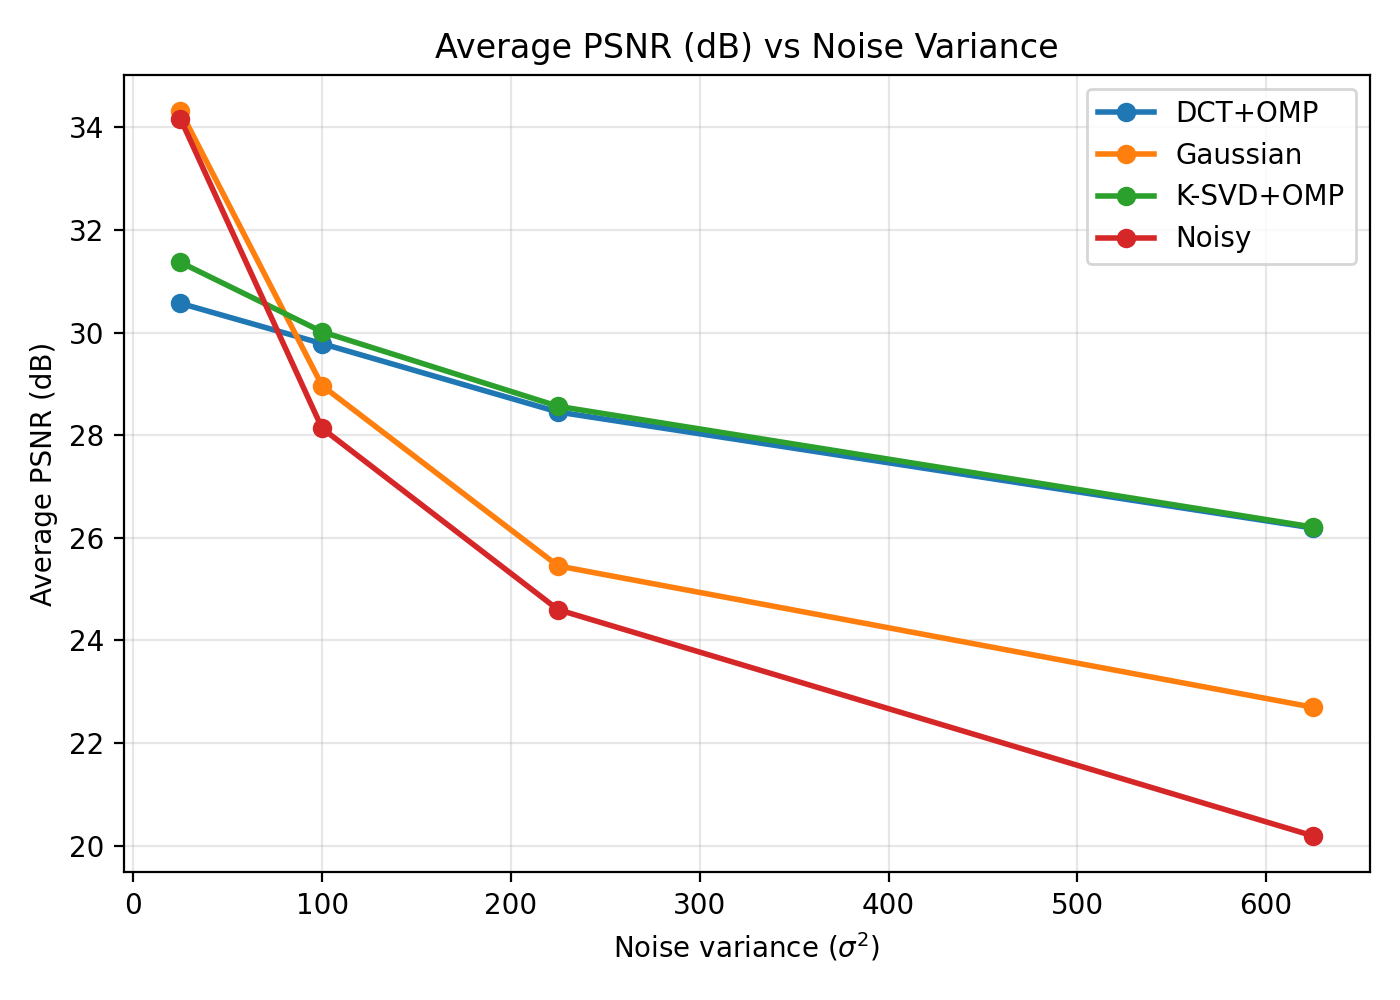
\includegraphics[width=0.72\textwidth]{fig_psnr_vs_noise_variance.png}
    \caption{Average PSNR versus noise variance for the four methods.}
    \label{fig:psnr_curve}
\end{figure}

\begin{figure}[H]
    \centering
    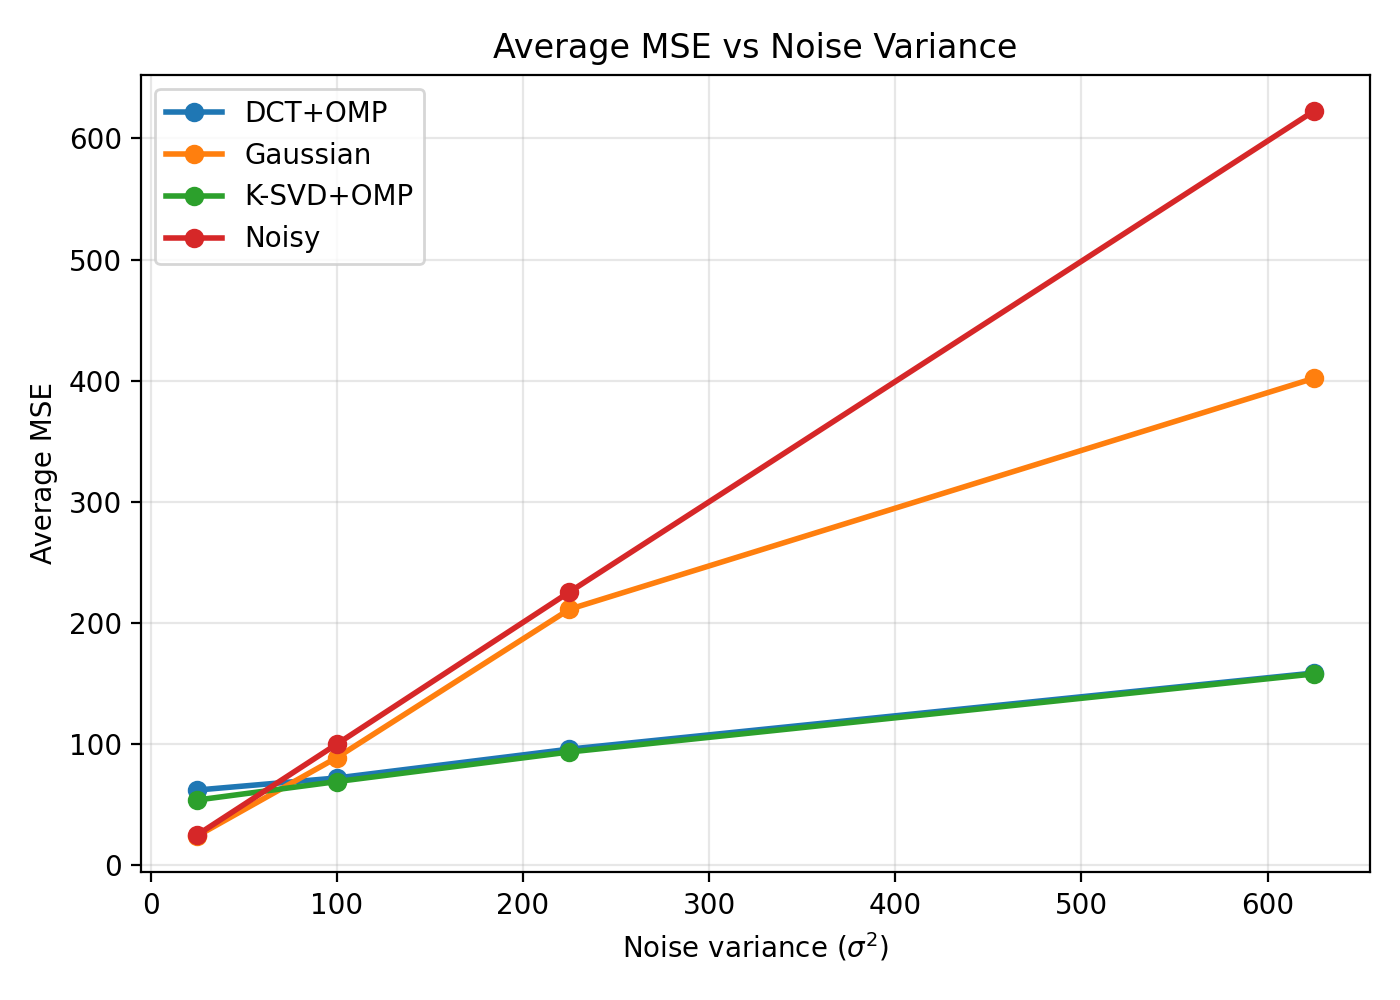
\includegraphics[width=0.72\textwidth]{fig_mse_vs_noise_variance.png}
    \caption{Average MSE versus noise variance for the four methods.}
    \label{fig:mse_curve}
\end{figure}

\begin{table}[H]
    \centering
    \caption{Average PSNR (dB) over the three selected images.}
    \label{tab:psnr}
    \begin{tabular}{ccccc}
        \toprule
        $\sigma$ & Noisy & Gaussian & DCT+OMP & K-SVD+OMP \\
        \midrule
        5  & 34.168 & 34.321 & 30.570 & 31.369 \\
        10 & 28.136 & 28.966 & 29.785 & 30.016 \\
        15 & 24.599 & 25.452 & 28.452 & 28.563 \\
        25 & 20.188 & 22.696 & 26.190 & 26.208 \\
        \bottomrule
    \end{tabular}
\end{table}

The results show that Gaussian filtering is competitive at very low noise ($\sigma = 5$), but sparse dictionary methods become clearly better as the noise level increases. K-SVD+OMP achieves the best average PSNR for $\sigma = 10$, $\sigma = 15$, and $\sigma = 25$. This is consistent with the expectation that a learned dictionary becomes more useful when the corruption is stronger.

\section{Qualitative Results}
Figure~\ref{fig:image1_all_sigmas} shows the denoising results for Image 1 across all four noise levels. This figure is useful for discussing how the relative strengths of the methods change as the noise increases.

\begin{figure}[H]
    \centering
    \begin{subfigure}{0.48\textwidth}
        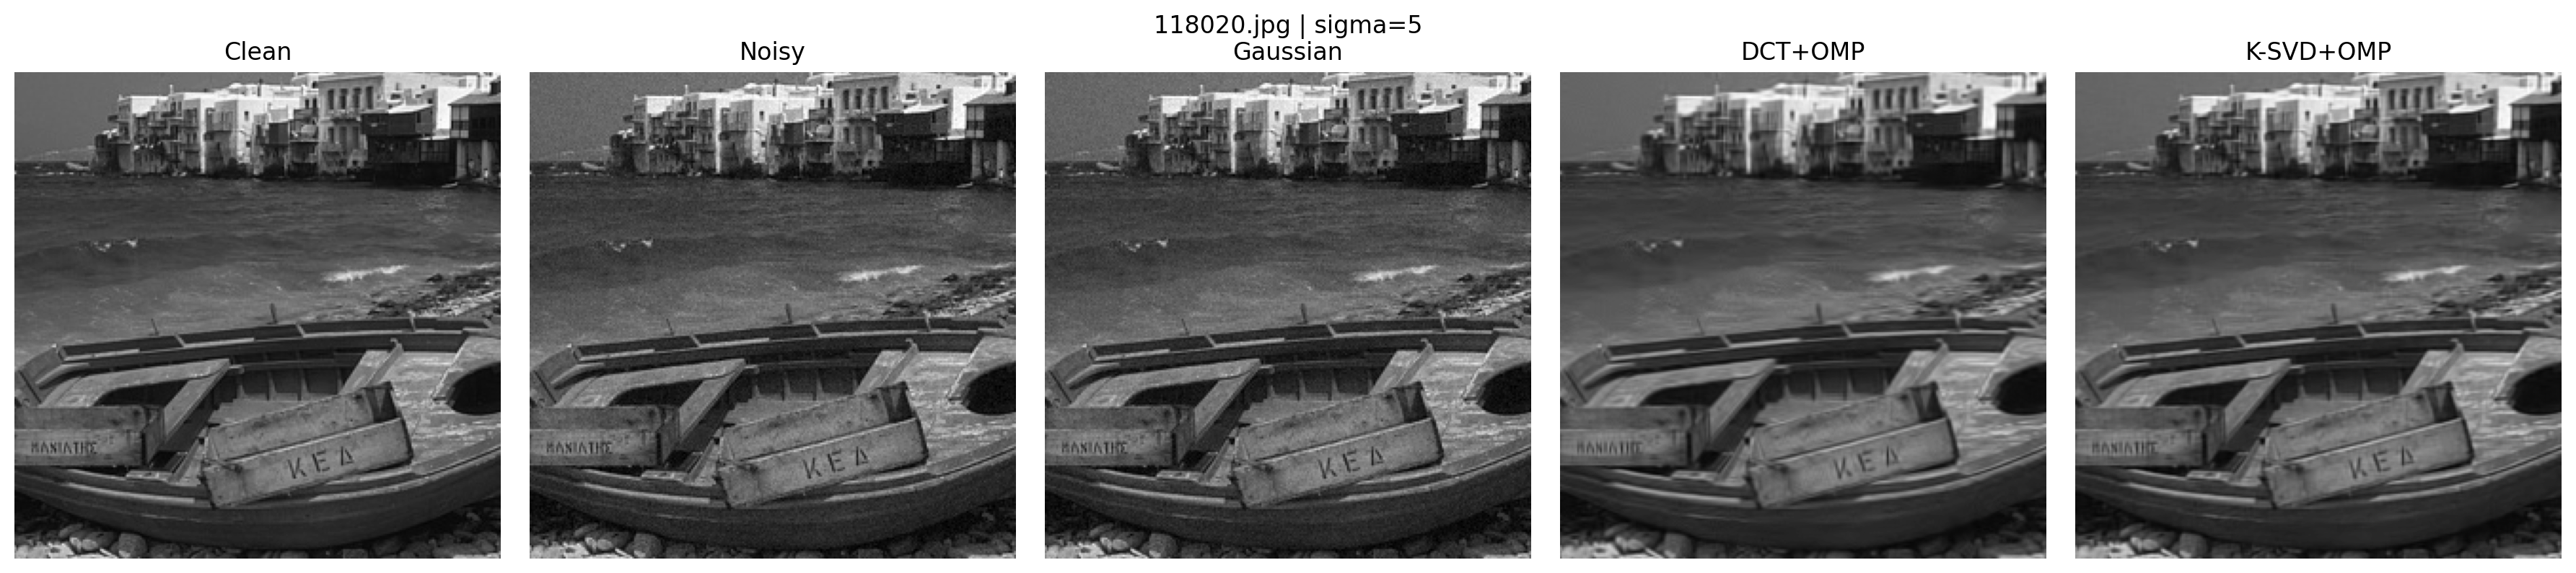
\includegraphics[width=\textwidth]{fig_comp_image1_sigma05.png}
        \caption{$\sigma = 5$}
    \end{subfigure}
    \hfill
    \begin{subfigure}{0.48\textwidth}
        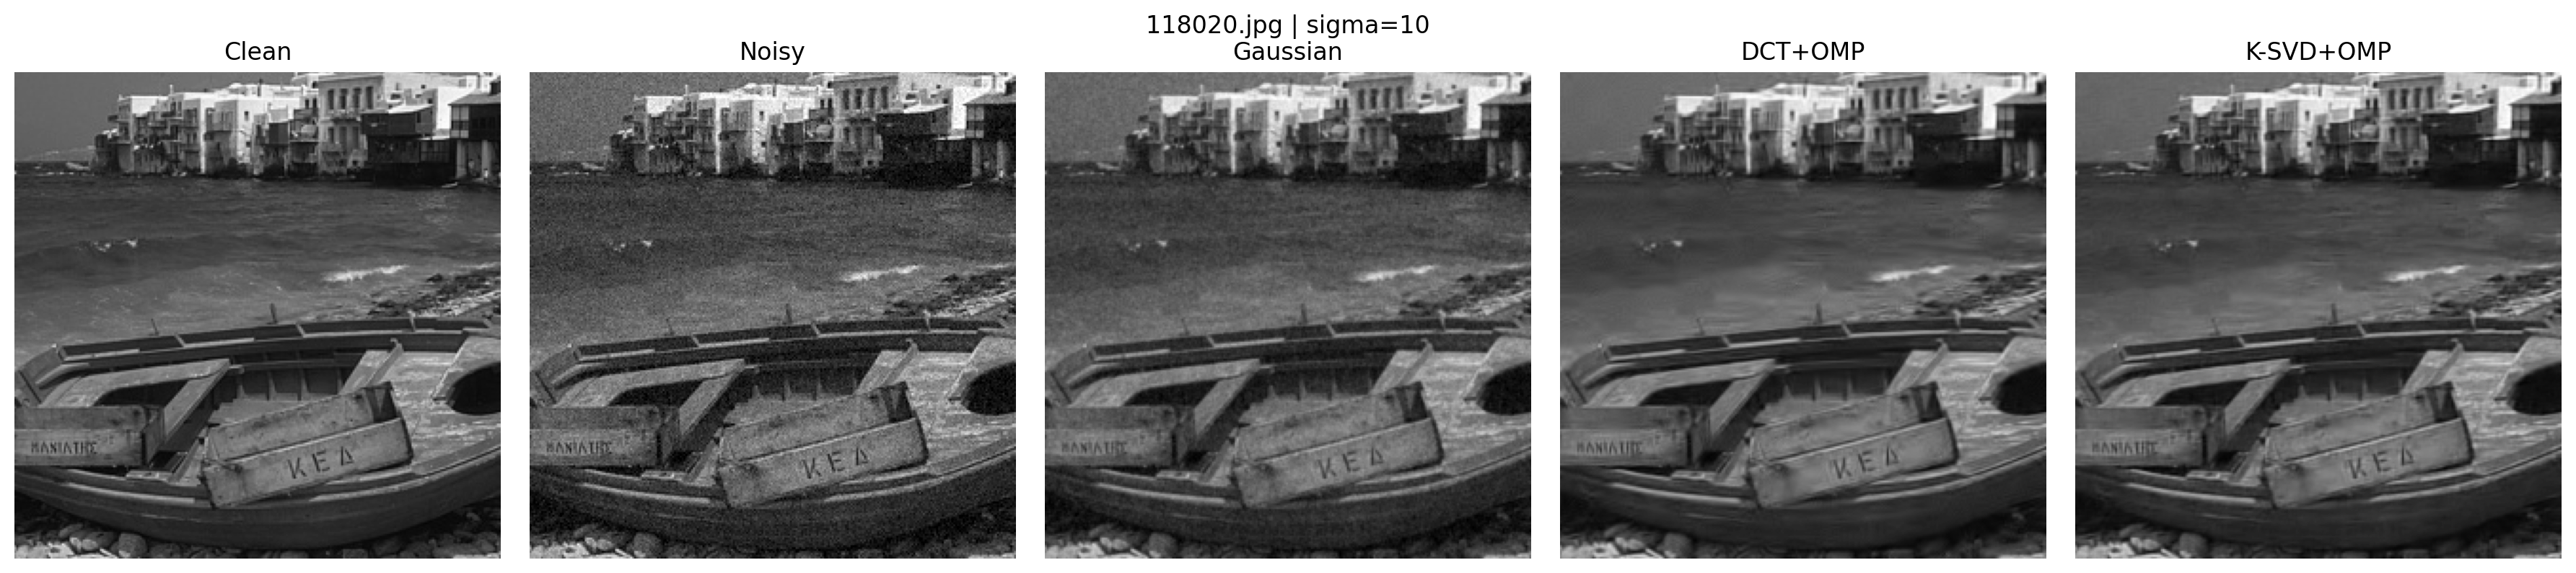
\includegraphics[width=\textwidth]{fig_comp_image1_sigma10.png}
        \caption{$\sigma = 10$}
    \end{subfigure}

    \vspace{0.5em}

    \begin{subfigure}{0.48\textwidth}
        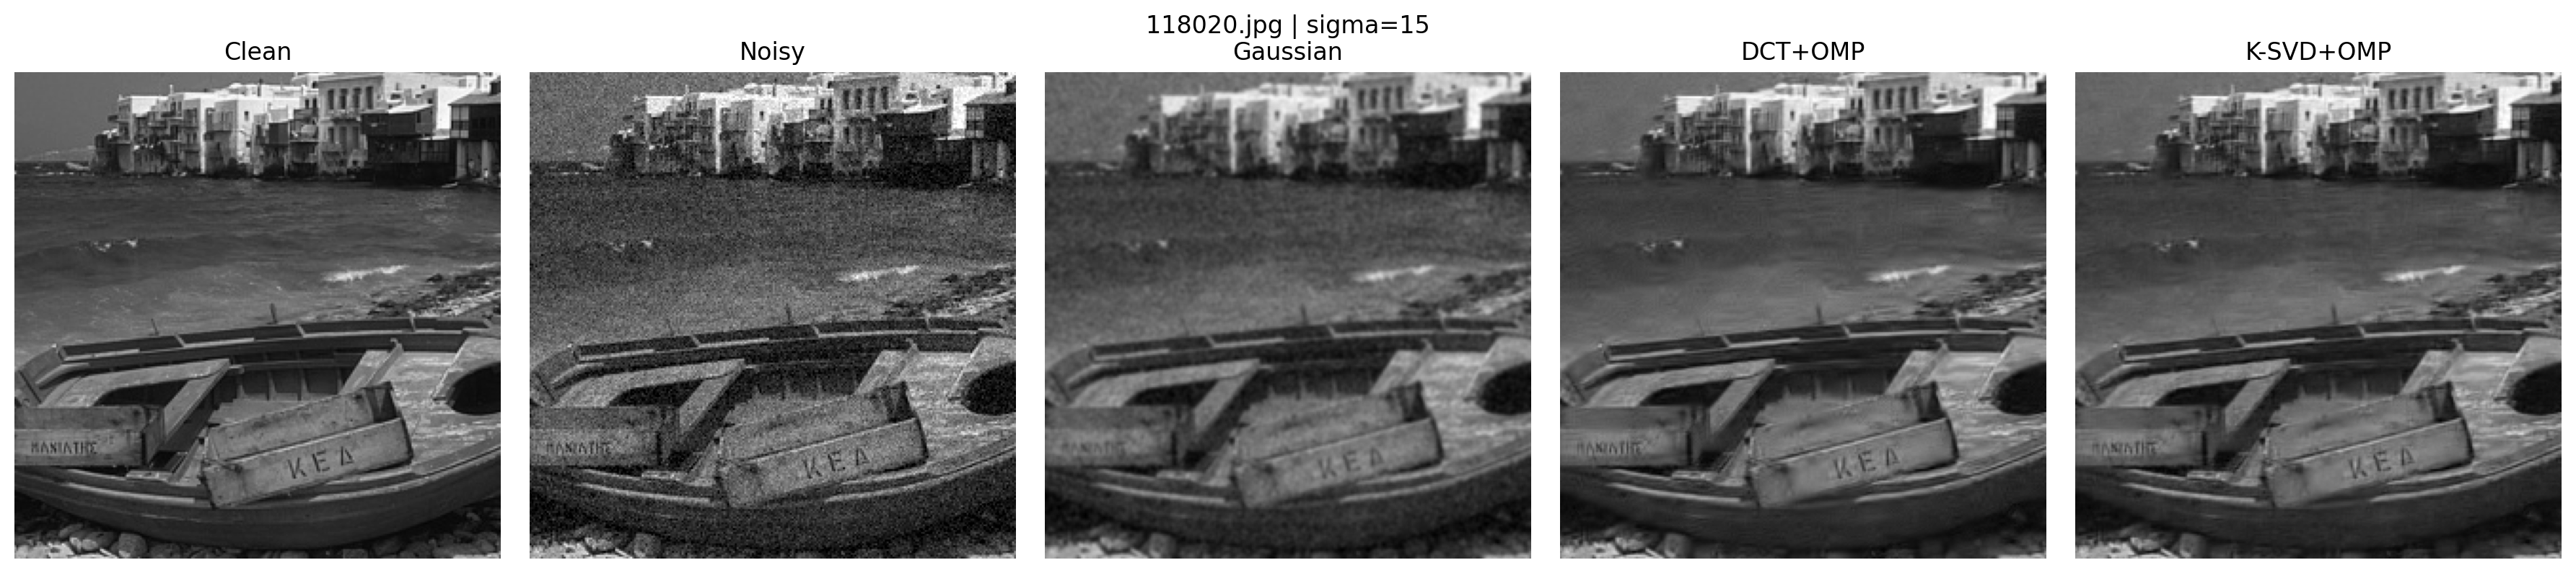
\includegraphics[width=\textwidth]{fig_comp_image1_sigma15.png}
        \caption{$\sigma = 15$}
    \end{subfigure}
    \hfill
    \begin{subfigure}{0.48\textwidth}
        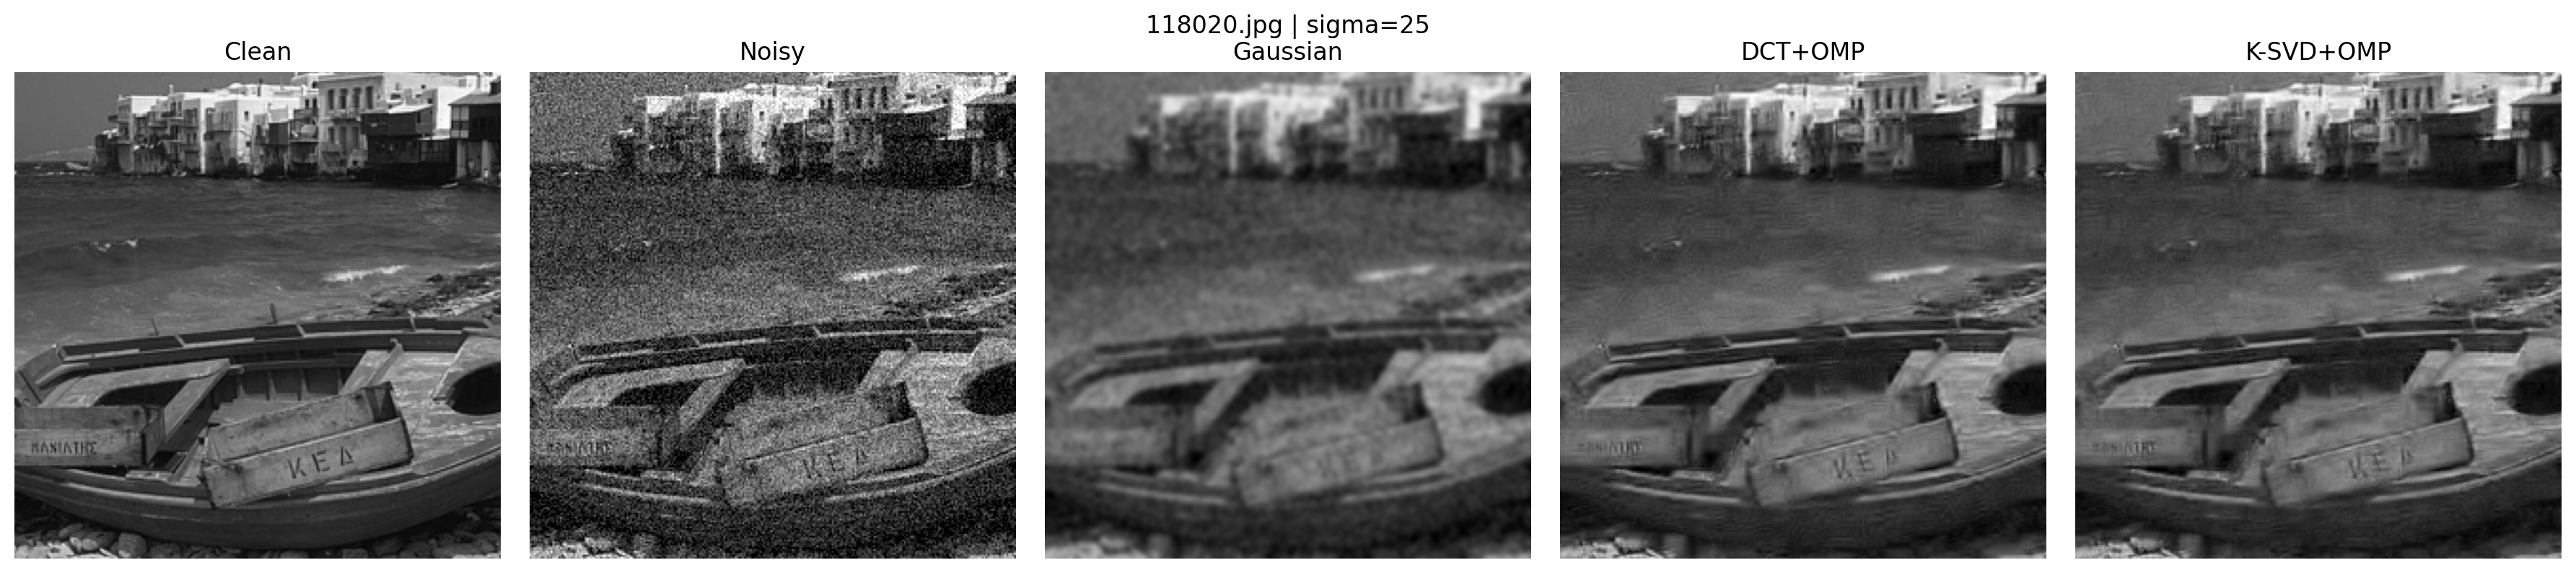
\includegraphics[width=\textwidth]{fig_comp_image1_sigma25.png}
        \caption{$\sigma = 25$}
    \end{subfigure}
    \caption{Visual comparison for Image 1 across all tested noise levels.}
    \label{fig:image1_all_sigmas}
\end{figure}

For completeness, Figures~\ref{fig:image2_sigma25} and \ref{fig:image3_sigma25} show the highest-noise case for the other two selected images. These examples highlight the robustness of sparse denoising at $\sigma = 25$.

\begin{figure}[H]
    \centering
    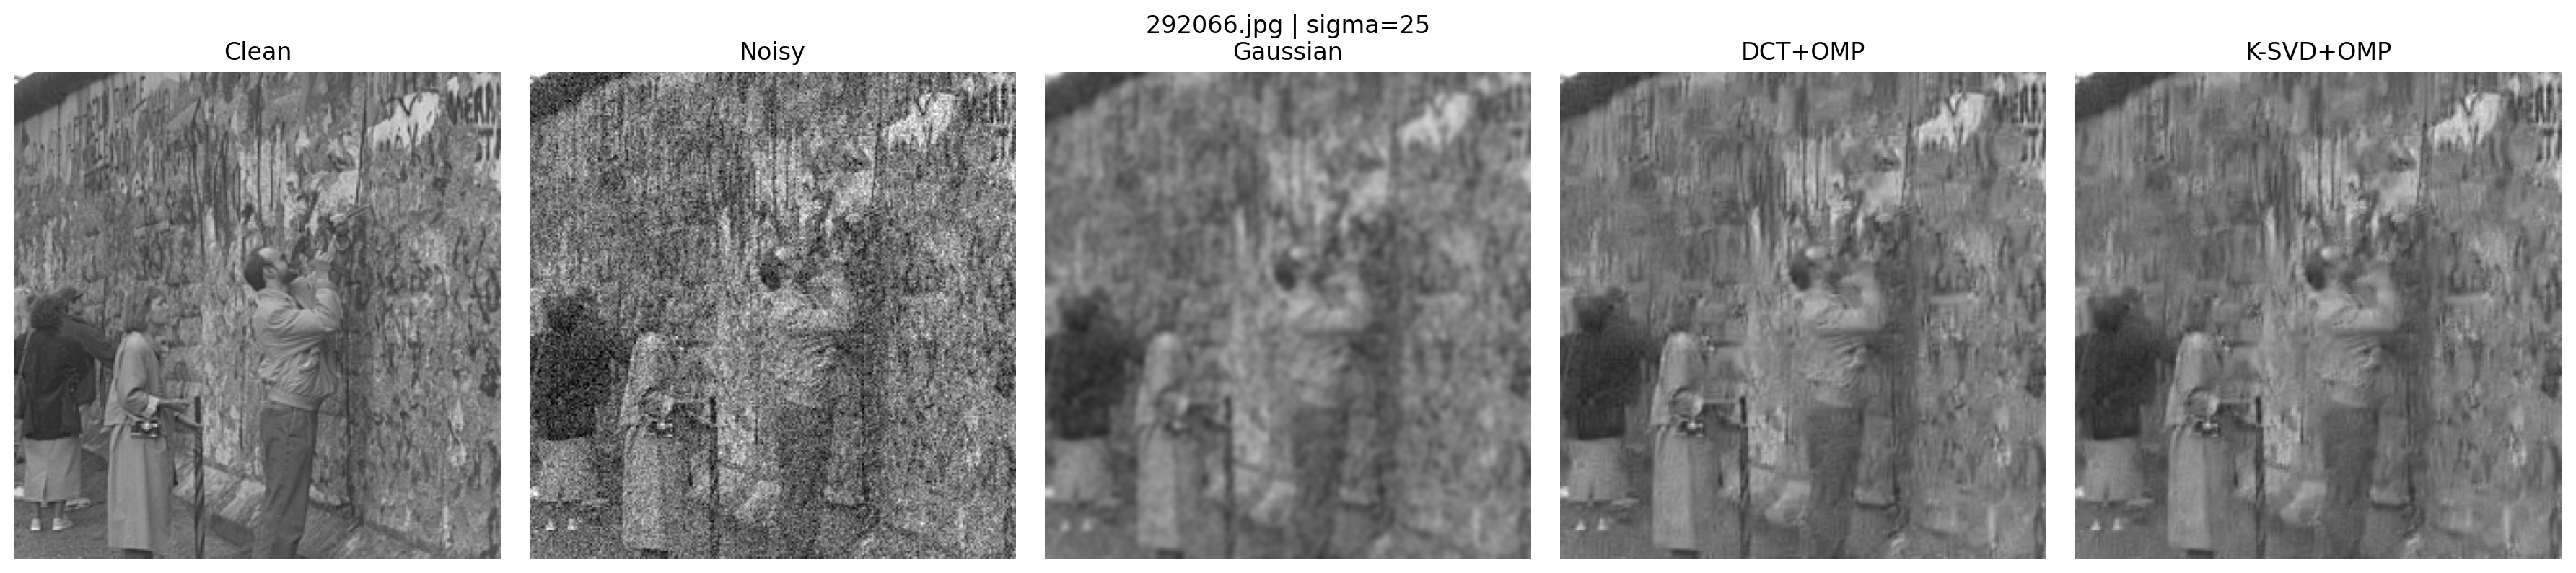
\includegraphics[width=0.82\textwidth]{fig_comp_image2_sigma25.png}
    \caption{Visual comparison for Image 2 at $\sigma = 25$.}
    \label{fig:image2_sigma25}
\end{figure}

\begin{figure}[H]
    \centering
    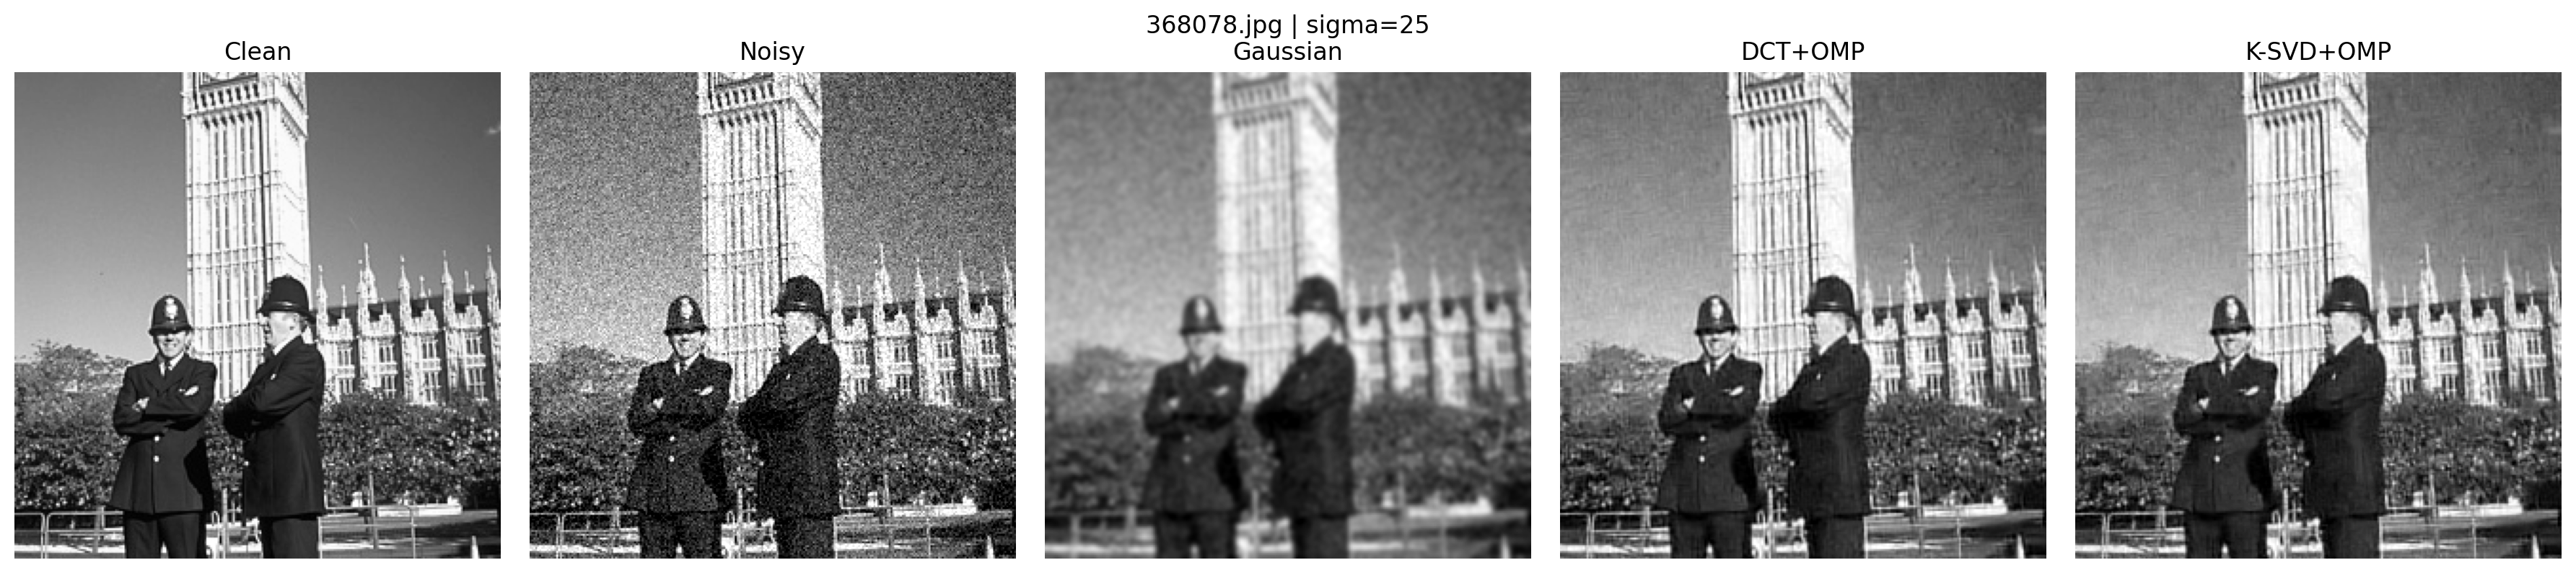
\includegraphics[width=0.82\textwidth]{fig_comp_image3_sigma25.png}
    \caption{Visual comparison for Image 3 at $\sigma = 25$.}
    \label{fig:image3_sigma25}
\end{figure}

\section{Learned Dictionary Visualization}
Figure~\ref{fig:dictionary} shows the learned dictionary atoms for Image 1 at $\sigma = 25$. The atoms resemble localized edges, gradients, and texture primitives, which is expected for natural-image patch modeling.

\begin{figure}[H]
    \centering
    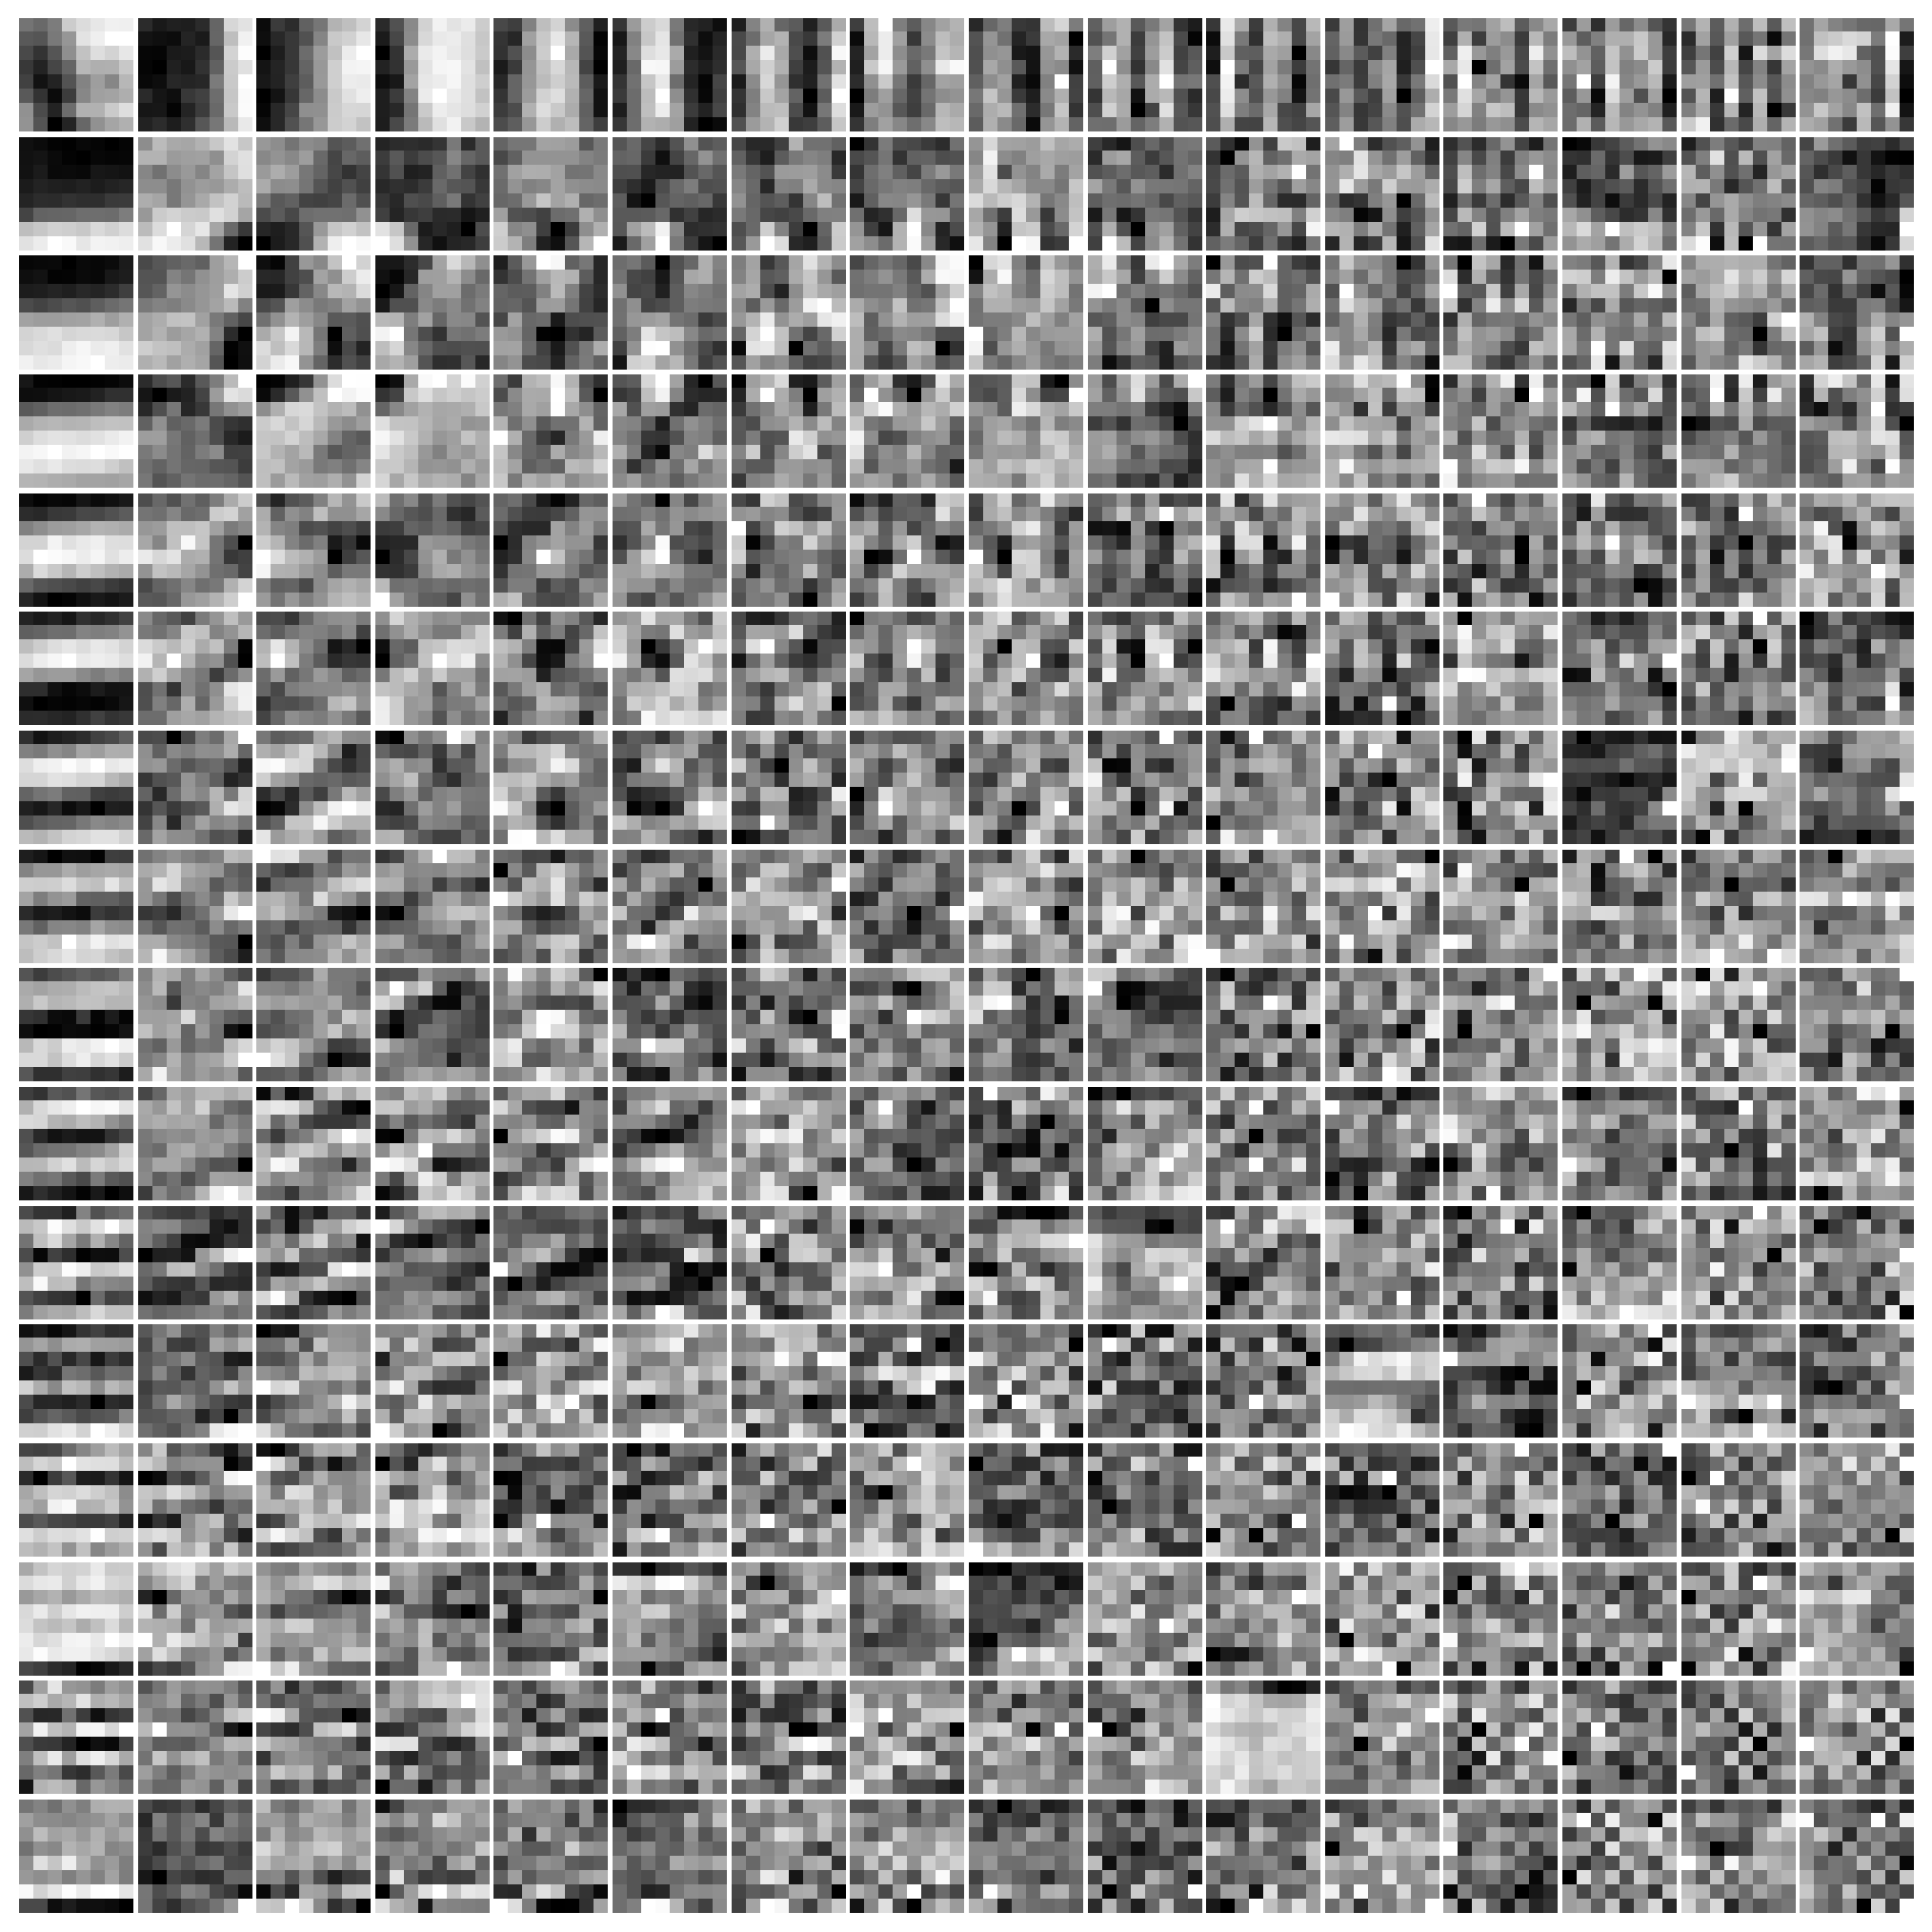
\includegraphics[width=0.58\textwidth]{fig_dictionary_image1_sigma25.png}
    \caption{Learned dictionary atoms for Image 1 at $\sigma = 25$.}
    \label{fig:dictionary}
\end{figure}

\section{Discussion}
The final results support the main motivation for dictionary learning. A fixed Gaussian smoother reduces noise but also blurs details, especially at higher noise levels. DCT+OMP improves the trade-off by exploiting sparse patch structure. K-SVD+OMP performs slightly better than DCT+OMP at most moderate and high noise levels because the dictionary is adapted to the image content rather than fixed in advance.

An interesting observation is that Gaussian filtering remains slightly better at $\sigma = 5$. This suggests that for weak corruption, the denoising problem is simple enough that a smooth low-pass baseline can already perform well, while sparse coding may introduce unnecessary reconstruction error. However, as the noise increases, the learned sparse model becomes more beneficial.

The report therefore satisfies the main experimental goal of studying error as a function of noise variance and comparing multiple denoising models under a common setup. A limitation is that only three images were used, so the conclusions should be interpreted as assignment-scale evidence rather than a large-scale benchmark. Another limitation is that the dictionary is learned from noisy patches of the same image, which is acceptable for image-adaptive denoising but should be stated explicitly.

\section{Conclusion}
This experiment shows that sparse dictionary learning is an effective approach for image denoising. Using the assignment configuration, K-SVD+OMP achieved the best average PSNR for three out of the four tested noise levels and consistently outperformed the noisy baseline at moderate and high noise levels. The results therefore support the use of learned overcomplete dictionaries for denoising natural images.

\begin{thebibliography}{9}

\bibitem{aharon2006ksvd}
M.~Aharon, M.~Elad, and A.~Bruckstein,
``K-SVD: An algorithm for designing overcomplete dictionaries for sparse representation,''
\emph{IEEE Transactions on Signal Processing},
vol.~54, no.~11, pp.~4311--4322, 2006.

\bibitem{fedorov2018multimodal}
I.~Fedorov and B.~D.~Rao,
``Multimodal sparse Bayesian dictionary learning,''
arXiv preprint arXiv:1804.03740, 2018.

\bibitem{joseph2020convergence}
G.~Joseph and C.~R.~Murthy,
``On the Convergence of a Bayesian Algorithm for Joint Dictionary Learning and Sparse Recovery,''
\emph{IEEE Transactions on Signal Processing},
vol.~68, pp.~343--358, 2020.

\end{thebibliography}

\end{document}
